\label{chap:political_sides}
Perspectives and Political Sides. What drives  the variations and propaganda? Which political interests? 

RQ:
How does political point of view influence the usage of propaganda?

\section{Propaganda across political spectrum}
4.3: comparison of sentiment/propaganda across political leaning

\section{Political leaning prediction using propaganda features}
5: political leaning classifier from propaganda features. Why


Why the two could benefit / be related?

The point of contact between political leaning prediction and propaganda is that both are dealing with political analysis.
Given that the facts that are being narrated are the same (exception: inclusion/exclusion), the main difference between an article from the left to one from the right is their point of view / subjective / persuasive component. Propaganda analysis is focused on analysing this specific component of the articles, the anti-topic model.
On this, we have our hypothesis that \emph{we can recognise the political leaning of an article by using the features provided by the propaganda analysis}.
The mixed analysis would allow to understand better why a certain article is classified as being left/right with respect to the black box BERT classifier.

The following sections first describe the general setup of the experiment, then deal with each one of the three research questions that we listed in the introduction: quantity, quantity by type, terms analysis.% TODO , context.


Unlike previous work on political leaning detection, in this paper we use a propaganda detection method (from \citet{da2019fine}) to identify the existence of propaganda and its type of technique in given articles, and incorporate this information directly as additional features into the training and testing of the model.  


\section{Other datasets for political leaning prediction}
6: classifier (propaganda → leaning) on other datasets

\section{Propaganda datasets are unbalanced}

8: propaganda datasets are unbalanced

\begin{figure}[!htb]
   \centering
   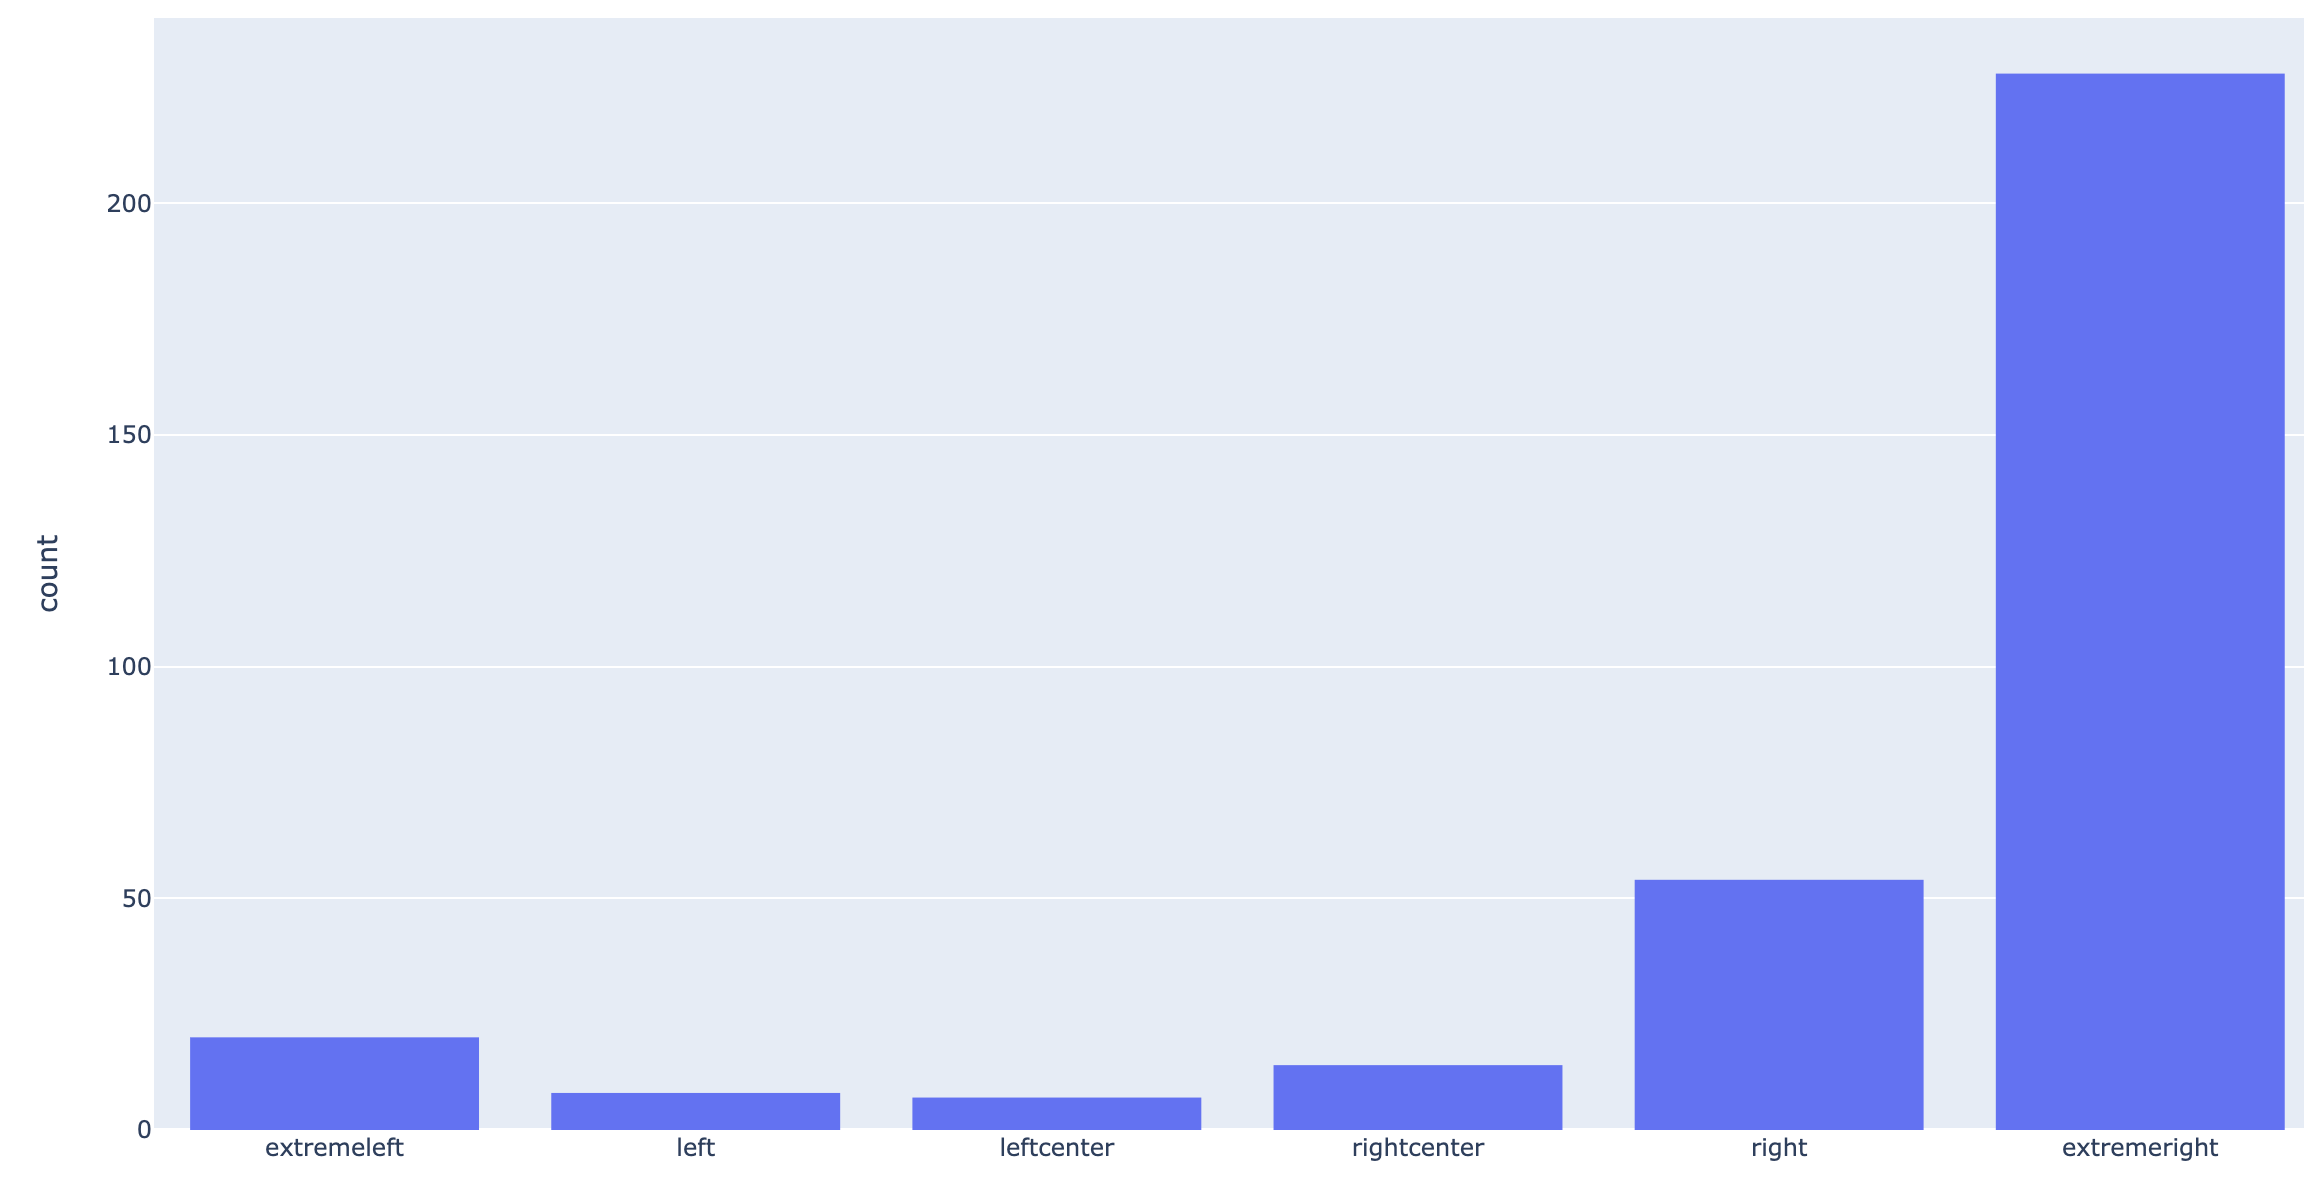
\includegraphics[width=\linewidth]{figures/leaning_questionable.png}
   \caption{The leaning of the propagandist sources from MBFC (TODO compare with effective training dataset, which is 100\% right)}
   \label{fig:mbfc_leaning}
\end{figure}

- Possible problems?
A possible problem of this approach that is not defended in the paper, is the choice of articles that have been annotated by experts. They have been selected from sources "propagandistic by Media Bias/Fact Check", in other words from the page \url{https://mediabiasfactcheck.com/fake-news/}. The propagandistic sources listed in this page, as Figure~\ref{fig:mbfc_leaning} shows, are mostly on the extreme-right side of the spectrum. Furthermore, the selection done by the authors (table 3 of that paper) results in all the sources of the articles to lean on the right.
So the resulting model is \textbf{being trained on very propagandistic sources from the right only}. The model will not be able to see left-propaganda because it never saw it in the training phase.

